\subsection{Serviço de Directoria -- OpenLDAP}

O \emph{LDAP}\footnote{Lightweight Directory Access Protocol} é o protocolo associado
a um serviço de directoria genérico que pode ser usado para armazenar praticamente todo
o tipo de informação.

Este protocolo define uma representação de dado hierárquica e, sendo um serviço de
directoria, é principalmente optimizado para operações de leitura em detrimento
das operações de escrita.
Na Figura~\ref{fig:ldap} pode-se observar um exemplo de uma hierarquia implementada
num servidor de LDAP.

\begin{figure}[H]
\begin{center}
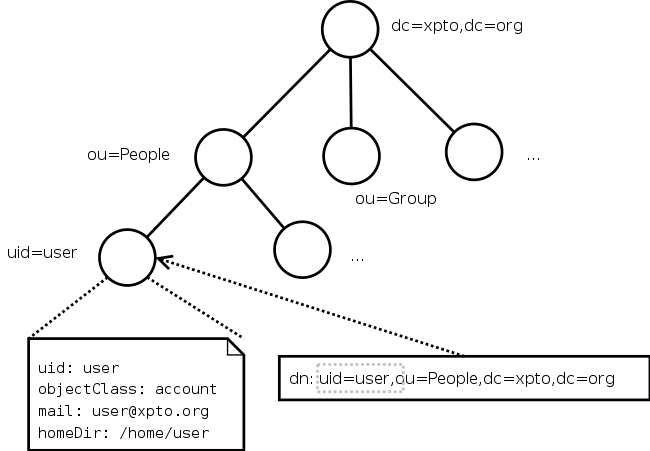
\includegraphics[width=10cm]{include/img/ldap}
\end{center}
\caption{Estrutura de uma árvore LDAP}
\label{fig:ldap}
\end{figure}

O ficheiro de configuração deste serviço é:

\texttt{/etc/openldap/slapd.conf}

Existem vários comandos para controlar este serviço:

\ServiceCommands{ldap}

